\documentclass[slovene,11pt,a4paper]{article}
\usepackage[margin=1.8cm,bottom=3cm,foot=1.5cm]{geometry}
\usepackage{amsmath}
\usepackage{booktabs}
\usepackage{float}
\usepackage{graphicx}
\usepackage{gensymb}
\usepackage{geometry}
\usepackage{changepage}
\usepackage{subcaption}
\usepackage{multirow}
\usepackage{blindtext}
\usepackage{hyperref}
\usepackage[slovene]{babel}
\pagenumbering{gobble}
\renewcommand{\contentsname}{\centering Contents}

\begin{document}

\title{3. naloga - Numerična minimizacija}
\author{Tadej Lozej 28201055}
\maketitle
\begin{center}
Modelska analiza 1 \\
\bigskip
Predavatelj: prof. dr. Simon Širca \\
Asistent: doc. dr. Miha Mihovilovič
\end{center}

\newpage

\tableofcontents

\newpage

\section{Uvod}

\pagenumbering{arabic}

V nalogi smo uporabljali različne algoritme numerične minimizacije za rešitev Thomsonovega problema in problema optimalne vožnje skozi semafor. Pri Thomsonovemu problemu na prevodno kroglo nanesemo $N$ enakih (klasičnih nabojev). Zanima nas kako se razmestijo po površini. Za reševanje tega problema smo uporabili več numeričnih metod minimizacije (\texttt{Nelder-Mead, Powell, CG, BFGS, L-BFGS-B, SLSQP}) in jih med seboj primerjali. Poleg krogle sem v nalogi pogledal tudi razmestitev nabojev po krogli v kondenzatorju, krogu, torusu in elipsoidu.

Z problemom optimalne vožnje smo se srečali že v prvi nalogi modelske analize 1. Tam smo ga rešili z variacijskih računom. V tej nalogi pa rešimo problem še z numerično minimizacijo in rezultata primerjamo.

\section{Tompsonov problem}

Pri Thomsonovem problemu na prevodno kroglo nanesemo $N$ enakih (klasičnih) nabojev. Zanima nas kako se ti razmestijo po površini. Zahevamo seveda minimum elektrostatične energije

\begin{equation}
W = \sum_{i, j>i} \frac{e_0^2}{4\pi\varepsilon_0 \Vert \vec{r_i}-\vec{r_j} \Vert} = \text{min},
\end{equation}
kjer je $e_0$ naboj klasičnega delca, $\vec{r_i}$ in $\vec{r_j}$ pa koordinati $i$-tega oz. $j$-tega delca. Elektrostatično energijo lahko prepišemo v brezdimenzijsko obliko z uvedbo brezdimenzijskih spremenljivk $\tilde{\vec{r_i}} = \vec{r_i}/r_0$ in energijo $\tilde{W} = 4\pi \varepsilon_0 r_0 / e_0^2 W$, kjer je $r_0$ radij krogle. Enačba (1) v brezdimenzijski obliki tako izgleda

\begin{equation}
W = \sum_{i, j>i} \frac{1}{\Vert \vec{r_i}-\vec{r_j} \Vert} = \text{min},
\end{equation}
kjer smo zaradi lažjega branja spustili $\tilde{}$. Energija je funkcija koordinat vseh nabojev.

\subsection{Sfera}

Kot prvi primer si poglejmo originalni Thomsonov problem. Iščemo razmestitev $N$ nabojev po površini prevodne krogle z minimizacijo elektrostatske energije. Želimo izraziti evklidsko razdaljo med dvema točkama na enotski sferi. Posamezne koordinate $x,y,z$ lahko izrazimo v sferičnem koordinatnem sistemu kot

\[
x_i = \sin\theta_i \cos\phi_i, \quad y_i = \sin\theta_i \sin\phi_i, \quad z_i = \cos\theta_i
\]
in evklidsko razdaljo med točkama $\vec{r_i} = (x_i, y_i, z_i)$ in $\vec{r_j} = (x_j, y_j, z_j)$ zapišemo kot

\begin{equation}
\Vert\vec{r_i}-\vec{r_j}\Vert = \sqrt{2-2\sin\theta_i\sin\theta_j\cos(\phi_i-\phi_j) - 2\cos\theta_i \cos\theta_j}.
\end{equation}
To razdaljo med dvema poljubnima točkama na enotski sferi nesemo v enačbo 2 in dobimo

\begin{equation}
W = \sum_{i, j>i} \frac{1}{\sqrt{2-2\sin\theta_i\sin\theta_j\cos(\phi_i-\phi_j) - 2\cos\theta_i \cos\theta_j}} = \text{min}.
\end{equation}
Elektrostatska energija na enotski sferi je tako funkcija $2N$ sferičnih koordinat vseh posameznih delcev $W = W(\phi_1, \theta_1, \phi_2, \theta_2,..., \phi_N, \theta_N)$. Pri nekaterih numeričnih metodah minimizacije lahko kot argument poleg same funkcije, ki jo želimo minimizirati podamo tudi njen gradient. To načeloma vodi do hitrejših in natančnejših rezultatov. Med omenjenimi metodami je to opcijo ponujajo metode \texttt{CG, BFGS, L-BFGS-B} in \texttt{SLSQP}. V nadaljevanju bomo primerjali te metode z podanim gradientom in brez podanega gradienta, zato izračunamo še gradient potencialne energije

\begin{equation}
\frac{\partial W}{\partial \phi_i} = \sum_{j, j\neq i} - \frac{\sin\theta_i \sin\theta_j \sin(\phi_i-\phi_j)}{(2-2\sin\theta_i \sin\theta_j \cos(\phi_i-\phi_j)-2\cos\theta_i \cos\theta_j)^{3/2}}
\end{equation}
in
\begin{equation}
\frac{\partial W}{\partial \theta_i} = \sum_{j, j\neq i} - \frac{\sin\theta_j \cos\theta_i \cos(\phi_i-\phi_j) - \cos\theta_j \sin\theta_i}{(2-2\sin\theta_i \sin\theta_j \cos(\phi_i-\phi_j)-2\cos\theta_i \cos\theta_j)^{3/2}}.
\end{equation}

Preden začnemo testirati numerične metode si za občutek poglejmo rešitve enačbe (4). Na spletni strani angleške wikipedije (\texttt{https://en.wikipedia.org/wiki/Thomson\_problem}) lahko dobimo podatke o elektrostatskih energijah Thomsonovega priblema v odvisnosti od števila nabojev na krogli. Brezdimenzijske energije so prikazane na sliki 1.

\begin{figure}[h!]
\centering
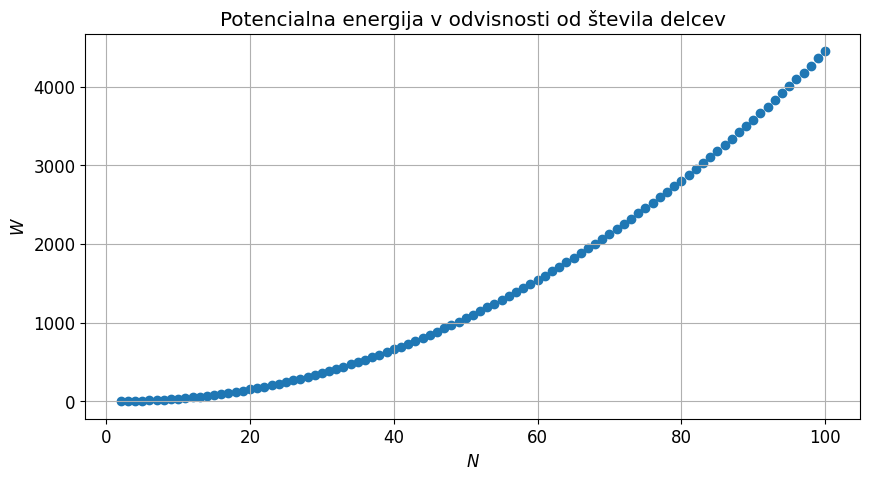
\includegraphics[width=12.5cm]{energije.png}
\caption{Potencialna energija v odvisnosti od števila delcev na krogli pri Thomsonovem problemu.}
\end{figure}

Prave vrednosti energij nam pridejo prav pri preverjanju natančnosti metod. Preverjene metode so \texttt{Nelder-Mead, Powell, CG, BFGS, L-BFGS-B} in \texttt{SLSQP}. Preverjal sem časovno zahtevnost, natančnost in število iteracij metod v odvisnosti od števila delcev na krogli. Rezultati so prikazani na sliki 2.

Na sliki vidimo, da metoda ja \texttt{Nelder-Mead} v večini primerov najmanj natančna in tudi precej počasna. Tudi število iteracij metode je precej večje v primerjavi z ostalimi. Metodi \texttt{BFGS} in \texttt{CG} sta najbolj natančni ampak tudi med časovno zahtevnejšimi. Metode \texttt{Powell, L-BFGS-B} in \texttt{SLSQP} so najhitrejše med testiranimi, vendar \texttt{Powell} očitno iztopa med tremi v manjši natančnosti in recej manjšem številu korakov.

Pri štirih natančnejših metodah lahko podamo tudi informacijo o gradientu v argumentu \texttt{jac} funkcije \texttt{scipy.optimize.minimize}. To storimo in opazujemo razlike med tem če gradient podamo ali ne. Rezultati za iste karakteristike kot prej so prikazani na sliki 3.

Vidimo, da matode s podanim gradientom niso precej natančnejše, so pa definitivno vse hitrejše.

\pagebreak 

\newpage
\begin{figure}[h!]
\centering
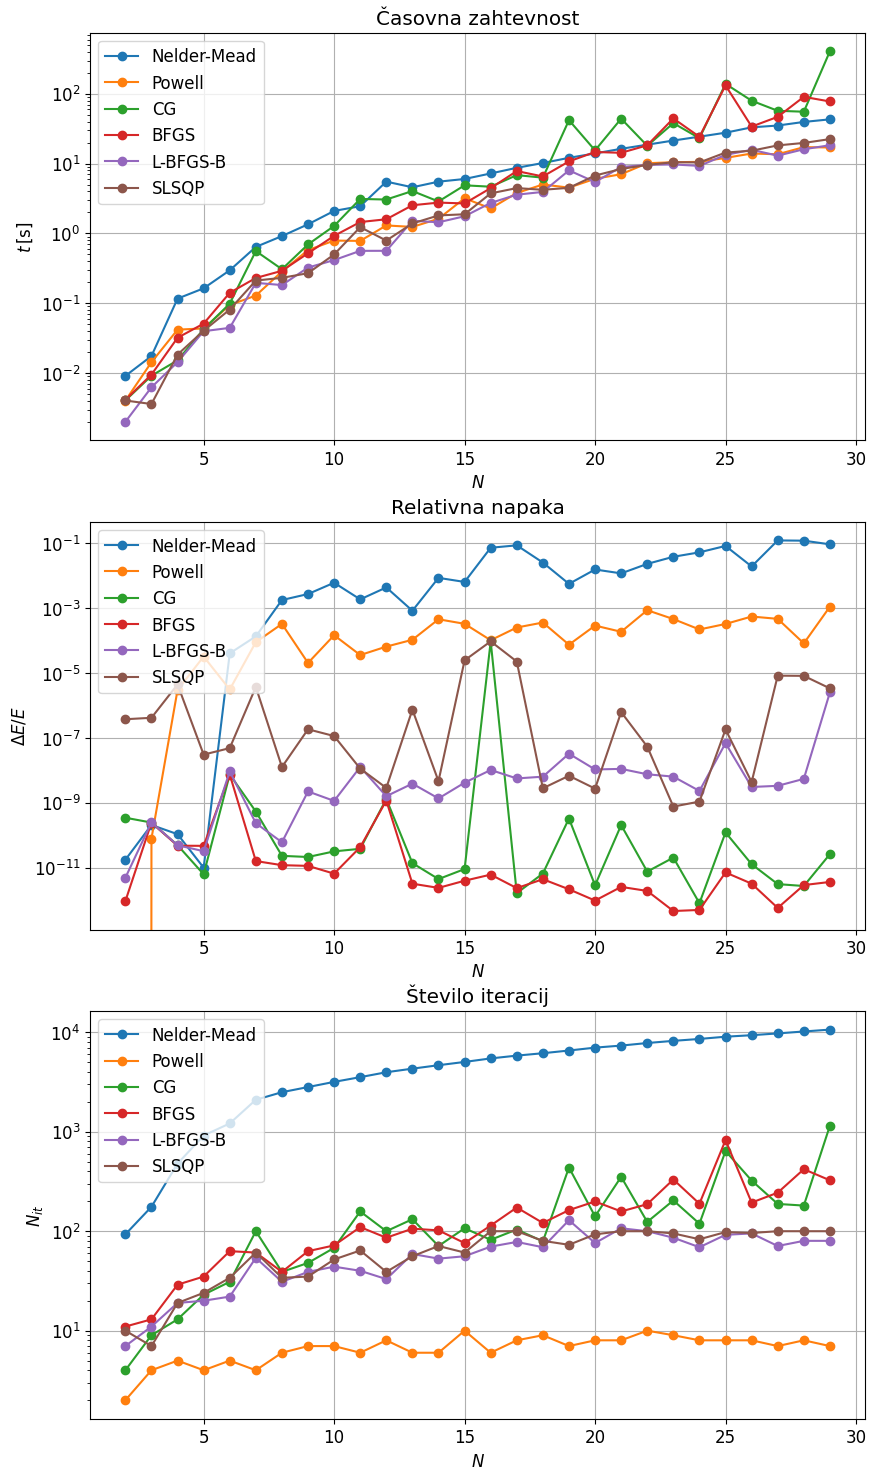
\includegraphics[width=12.5cm]{metode.png}
\caption{Primerjava različnih numeričnih metod minimizacije med seboj. Z metodami rešujemo Thomsonov problem pri različnem številu delcev na sferi. Grafi prikazujejo časpvno zahtevnost, relativno napako in število iteracij metod \texttt{Nelder-Mead, Powell, CG, BFGS, L-BFGS-B} in \texttt{SLSQP}.}
\end{figure}

\newpage
\begin{figure}[h!]
\centering
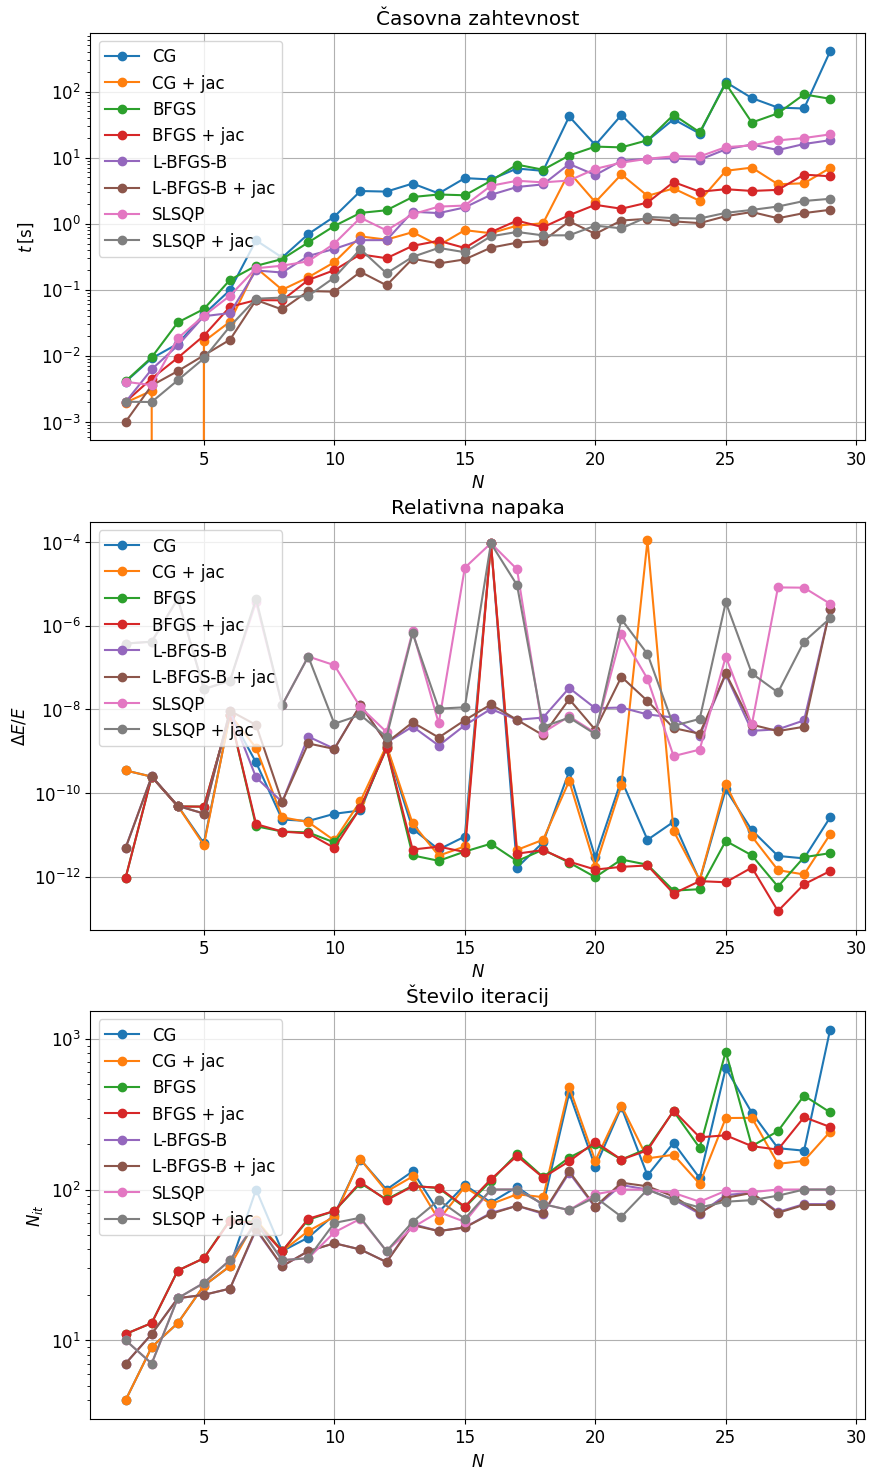
\includegraphics[width=12.5cm]{metode2.png}
\caption{Primerjava različnih numeričnih metod minimizacije med seboj. Z metodami rešujemo Thomsonov problem pri različnem številu delcev na sferi. Grafi prikazujejo časpvno zahtevnost, relativno napako in število iteracij metod \texttt{CG, BFGS, L-BFGS-B} in \texttt{SLSQP} z podanim gradientom in brez.}
\end{figure}

\newpage

Zaradi natančnosti te metode sem se odločil, da bom nadaljne probleme reševal z \texttt{BFGS}. Na sliki 4 za različno število nabojev $N$ prikažemo razmestitev le-teh na sferi. Za prvih nekaj $N$ vidimo, da se delci razporedijo po sferi v precej lepo vidne oblike.

\begin{figure}[h!]
\centering
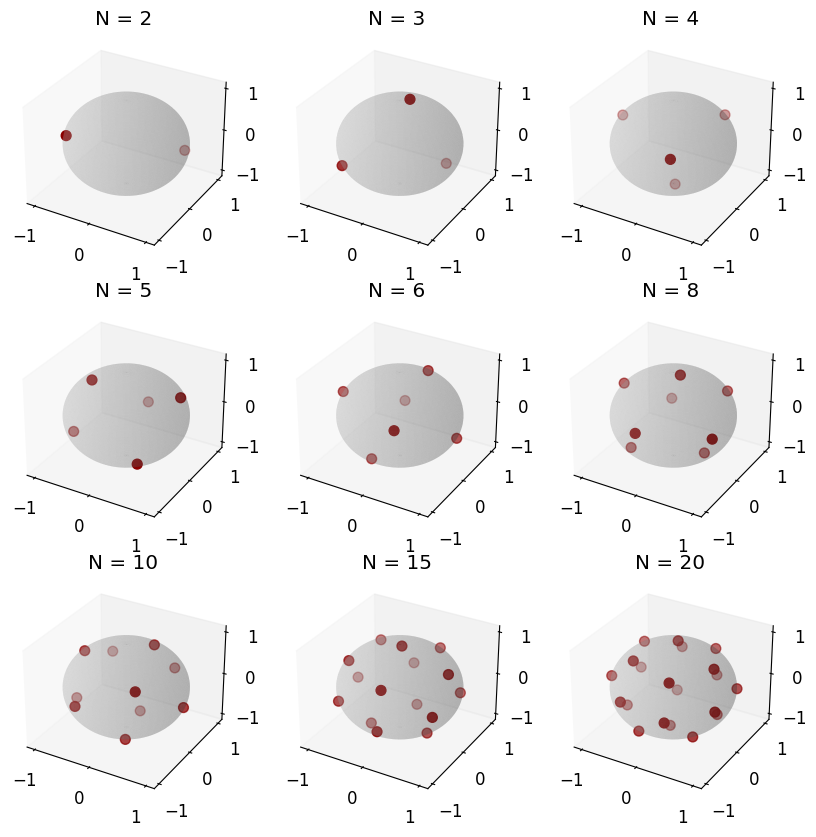
\includegraphics[width=12.5cm]{sfera.png}
\caption{Razmestitve $N$ delcev na enotski sferi.}
\end{figure}

\subsection{Sfera v kondenzatorju}

Kako se delci razporedijo po sferi in kakšne so elektrostatske energije če sfero postavimo v homogeno električno polje oz. kondenzator. V zapisu energije sistema dobimo dodaten člen $-eEx$ zaradi kondenzatorja

\begin{equation}
W = \sum_{i, j>i} \frac{e_0^2}{4\pi\varepsilon_0 \Vert \vec{r_i}-\vec{r_j} \Vert}
- \sum_i e_0Ez_i = \text{min},
\end{equation}
kjer je E jakost električnega polja. Električno polje je usmerjeno v smeri $\hat{e_z}$ in naboji na sferi zo pozitivni. Efektivno smo utežili koordinato z. Delci bodo silili k večji vrednosti z, saj jih tja sili električno polje. Z ponovno uvedbo brezdimenzijskih spremenljivk $\tilde{\vec{r_i}} = \vec{r_i}/r_0$, $\tilde{W} = 4\pi \varepsilon_0 r_0 / e_0^2 W$, $\tilde{E} = 4\pi \varepsilon_0 r_0^2 / e_0 E$ in $\tilde{z_i} = z_i-r_0$, kjer je $r_0$ radij krogle je brezdimenzijska energija

\begin{equation}
W = \sum_{i, j>i} \frac{1}{\Vert \vec{r_i}-\vec{r_j} \Vert} - E \sum_i z_i = \text{min}.
\end{equation}
Enačbo minimiziramo pri vrednosti $E=10$ in dobimo za nekaj $N$ izrišemo razmestitev nabojev po sferi. Na sliki 5 so prikazani rezultati. Vidimo, da delci silijo k večji vrednosti koordinate $z$.

\begin{figure}[h!]
\centering
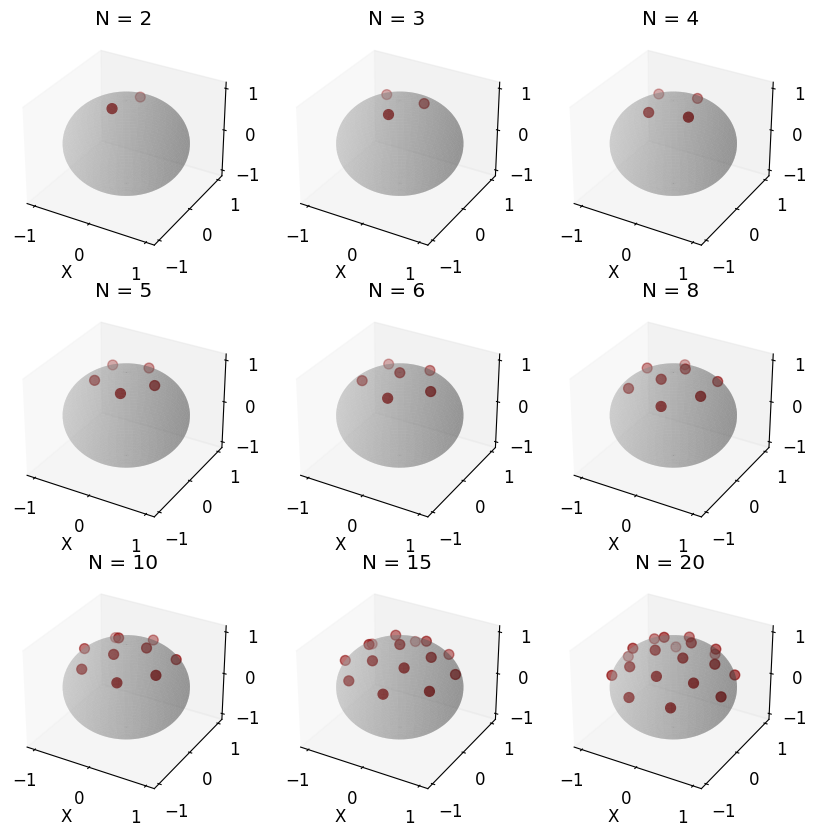
\includegraphics[width=12.5cm]{sfera2.png}
\caption{Razmestitve $N$ delcev na enotski sferi v kondenzatorju.}
\end{figure}

\subsection{Krog}

Poglejmo si še kakšne druge like in telesa na katerih lahko izračunamo razmestitev nabojev z minimizacijo potencialne energije. Poglejmo si minimizacijo potencialne energije na enotskem krogu. V podobnem stilu kot v podpoglavju 2.1. izračunajmo evklidsko razdaljo med dvema poljubnima točkama na enotskem krogu

\[
x_i = r_i \cos\phi, \quad y_i = r_i \sin\phi_i
\]
in evklidsko razdaljo med točkama $\vec{r_i} = (x_i, y_i)$ in $\vec{r_j} = (x_j, y_j)$ zapišemo kot

\begin{equation}
\Vert\vec{r_i}-\vec{r_j}\Vert = \sqrt{r_i^2 + r_j^2 - 2r_ir_j \cos(\phi_i-\phi_j)}.
\end{equation}
Brezdimenzijska elektrostatska energija je v tem primeru

\begin{equation}
W = \sum_{i, j>i} \frac{1}{\sqrt{r_i^2 + r_j^2 - 2r_ir_j \cos(\phi_i-\phi_j)}}.
\end{equation}
Ko to minimiziramo prikažemo rezultate za nekaj $N$ nabojev na enotskem krogu na sliki 6.

\newpage

\begin{figure}[h!]
\centering
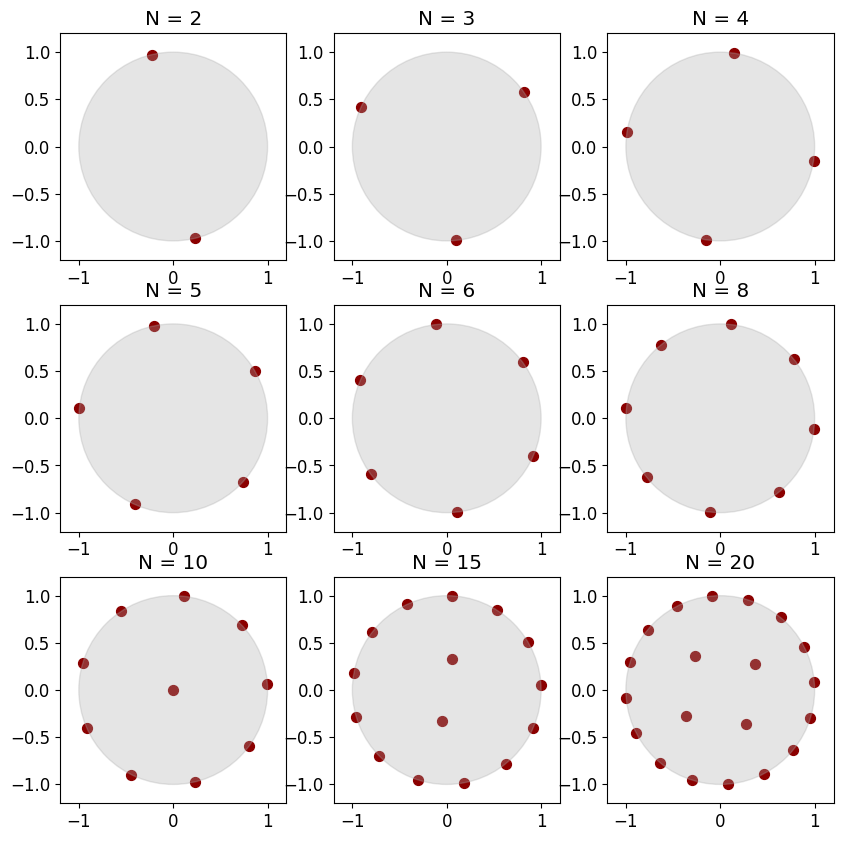
\includegraphics[width=12.5cm]{krog.png}
\caption{Razmestitve $N$ delcev na enotskem krogu.}
\end{figure}

\subsection{Torus}

Za razmestitev delcev na torusu z velikim premerom $R=1$ ga parametriziramo s kotoma $\theta$ in $\phi$. Mesto $i$-tega naboje se nahaja na koordinatah 

\[
x_i = (1+r\cos\theta_i)\cos\phi_i, \quad y_i = (1+r\cos\theta_i)\sin\phi_i, \quad z_i = r\sin\theta_i,
\]
kjer je $r$ mali premer torusa. Pri izračunu razmestitve vzamemo $r=0.25$. V tem primeru je prenaporno poenostaviti izraz za evklidsko razdaljo med dvema poljubnima točkama na torusu, zato prvo izračunamo koordinate nabojev in nato razdaljo med njima. Ustrezno izračunamo evklidsko razdaljo med dvema poljubnima točkama na torusu $\vec{r_i} = (x_i, y_i, z_i)$ in $\vec{r_j} = (x_j, y_j, z_j)$ ter prikažemo rezultate za nekaj $N$ na sliki 7. Vidimo, da kot pričakovano se delci nabirajo na zunanji strani torusa, da vzdržujejo čim večjo razdaljo med seboj.

\newpage

\begin{figure}[h!]
\centering
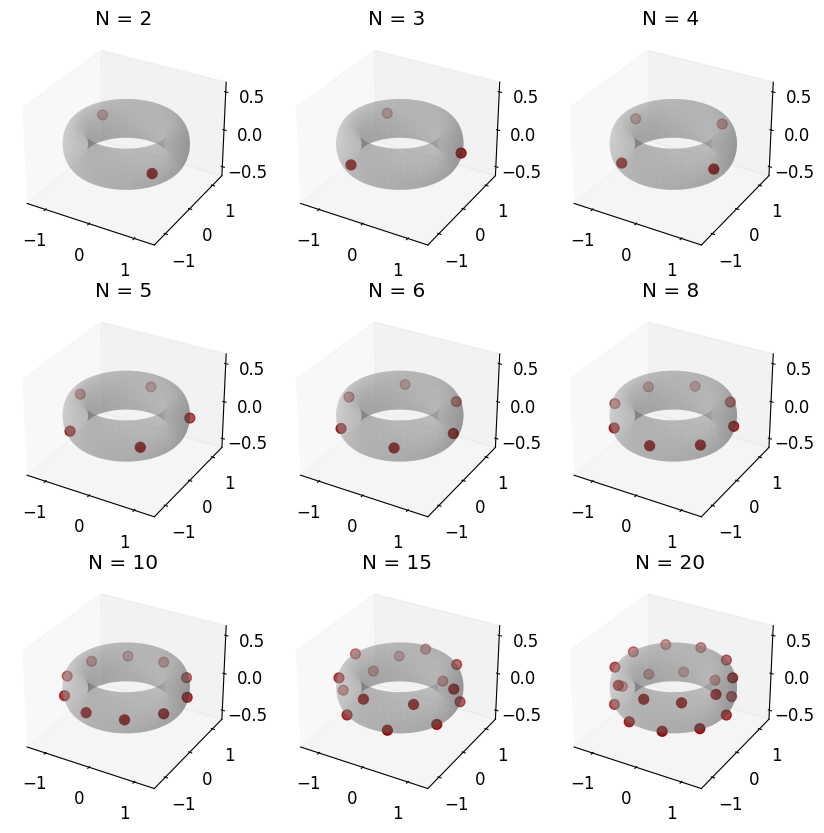
\includegraphics[width=12.5cm]{torus.png}
\caption{Razmestitve $N$ delcev na torusu z velikim radijem $R=1$ in malim radijem $r=0.25$.}
\end{figure}

\subsection{Elipsoid}

Zelo podobno kot za torus lahko dobimo razmestitev nabojev po elipsoidu. Mesta nabojev parametriziramo z dvema kotoma $\phi$ in $\theta$. Na elipsoidu z polosjo $a=1$ vzdolž $x$ parametriziramo $i$-ti naboj kot

\[
x_i = \sin\theta_i \cos\phi_i, \quad y_i = b\sin\theta_i\sin\phi_i, \quad z_i = c\cos\theta_i,
\]
kjer sta $b$ in $c$ polosi v smereh $y$ in $z$. Pri izračunu razmestitve delcev si izberemo $b=0.5$ in $c=0.8$. Podobno kot pri torusu je tudi tukaj prenaporno  poenostaviti izraz za evklidsko razdaljo med dvema poljubnima točkama, zato prvo izračunamo koordinate dveh delcev in nato evklidsko razdaljo med njima. Ustrezno izračunamo evklidsko razdaljo med dvema poljubnima točkama na elipsoidu $\vec{r_i} = (x_i, y_i, z_i)$ in $\vec{r_j} = (x_j, y_j, z_j)$ ter prikažemo rezultate za nekaj $N$ na sliki 8.

\newpage

\begin{figure}[h!]
\centering
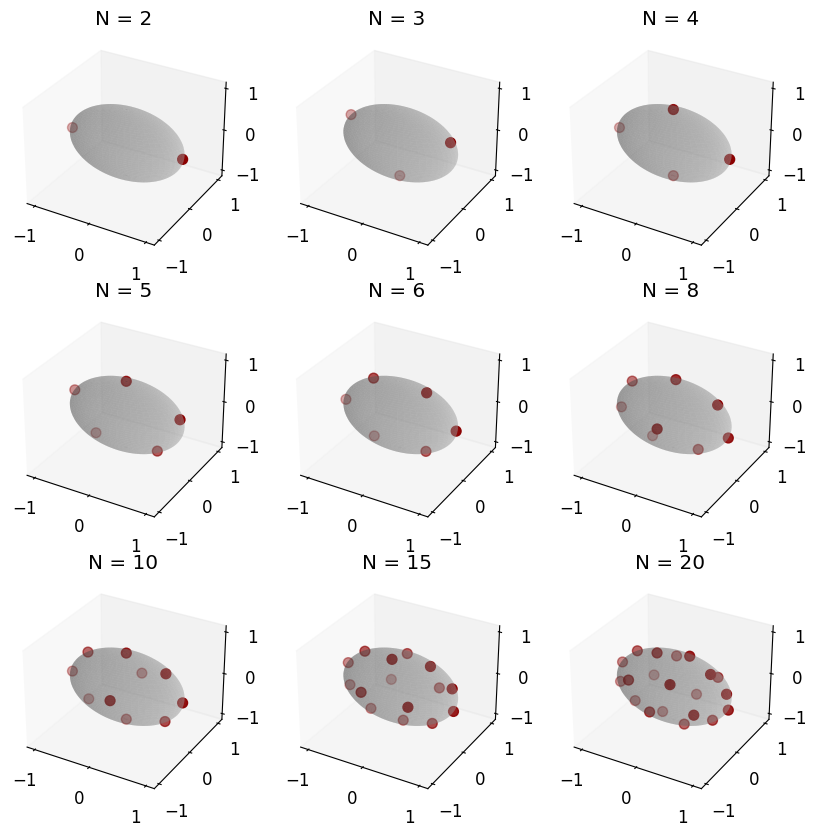
\includegraphics[width=12.5cm]{elipsoid.png}
\caption{Razmestitve $N$ delcev na elipsoidu z polosmi $a=1$, $b=0.5$ in $c=0.8$.}
\end{figure}

\subsection{Primerjava teles in likov}

Za vsa omenjena telesa in like si poglejmo elektrostatsko energijo v odvisnosti od števila nabojev na telesu oz. liku. Reultati so prikazani na sliki 9. Izkaže se, da je izmed izbranih teles in likov za majhne $N$ najbolj ugodno polagati naboje na torus, za večje $N$ pa na sfero. To je zato, ker dokler je na telesu malo delcev so za izbran torus povprečne razdalje med njimi večje kot na sferi. Ko na telo nanesemo več delcev pa pri sferi pride upoštev njena večja raztegnjenost v smeri $z$ osi. Izbrani elipsiod se kljub njegovim trem dimenzijam izkaže manj ugoden kot krog. Oba sta pa seveda manj ugodna kot torus in sfera. Rezultat sfere v kondenzatorju moramo vzeti z rezervo, saj je načeloma odbojna energija med delci večja kot pri ostalih rezultatih.

\newpage

\begin{figure}[h!]
\centering
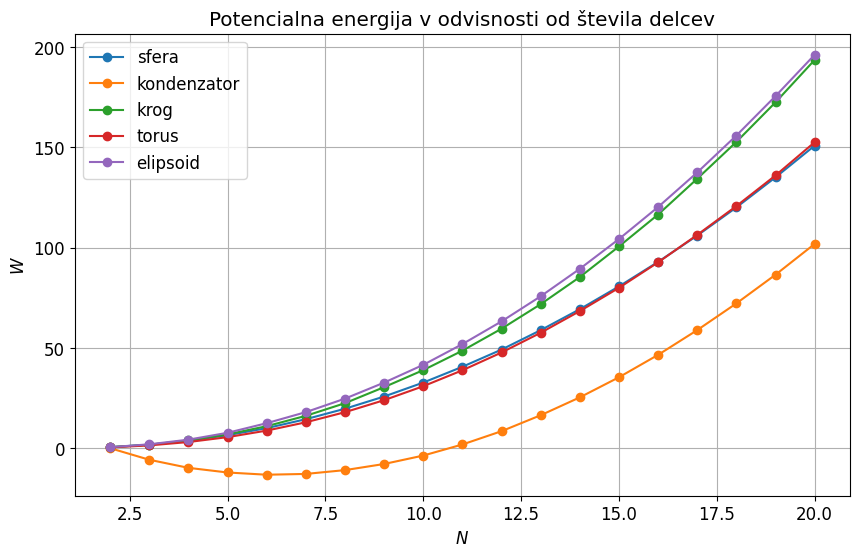
\includegraphics[width=12.5cm]{energije2.png}
\caption{Potencialna energija v odvisnosti od števila delcev na krogli, krogli v kondenzatorju, krogu, torusu in elipsoidu}
\end{figure}

\section{Problem optimalne vožnje}

Problem optimalne vožnje, ki smo ga srečali že v prvi nalogi, kjer smo ga reševali z variacijskim računom, lahko rešujemo tudi z numerično minimizacijo, če časovno skalo diskretiziramo. Minimiziramo funkcional

\begin{equation}
F = \int \left( \frac{d\nu}{d\tau} \right)^2 d\tau = \text{min},
\end{equation}
ki ga moramo za reševanje z numerično minimizacijo prepisati v diskterno obliko. To storimo z trapezno furmulo za numerično integracijo. Naš časovni interval razdelimo na $N$ diskretnih točk $\tau_i$ na razdalji $\Delta\tau$. Funkcional v diskretni obliki je

\begin{equation}
F_0 = \frac{1}{2} \left( \frac{\nu_0}{\Delta \tau} \right)^2 + \sum_{i=1}^{N-1} \left( \frac{\nu_i - \nu_{i-1}}{\Delta \tau} \right)^2 + \frac{1}{2} \left( \frac{\nu_N - \nu_{N-1}}{\Delta \tau} \right)^2.
\end{equation}

Pogoj o prevoženi razdalji v določenem času lahko dosežemo z manipulacijo funkcionala. Lahko mu dodamo člene in s tem silimo k upoštevanju željenih pogojev oz. vezi. Funkcionalu $F_0$ lahko prištejemo pogoj $F_1$

\begin{equation}
F_1 = 1 + e^{\kappa_1 \left( \frac{1}{2} \nu_0 + \sum_{i=1}^{N-1} \nu_i + \frac{1}{2} \nu_N - N \right)}
\end{equation}
in ga tako pri minimizaciji prisilimo k rešitvam, ki ustrezajo pogoju o prevoženi poti v določenem času. Minimiziramo funkcijo

\begin{equation}
F = F_0 + F_1 = \text{min}.
\end{equation}

Slika 10 prikazije rezultate te minimizacije pri različno fino nadrobljenem časovnem intervalu (vrednost $N$). Na sliki je z rdeču črto prikazana tudi teoretična rešitev iz naloge 1. Za začetno hitrost sem izbral $\nu_0 = 1$ in parameter $\kappa_1$ sem nastavil na $10$. Že pri tej vrednosti sem imel težave z velikimi vrednostmi eksponenta v $F_1$ zato nisem želel pogoja zastaviti še strožje.

\newpage

\begin{figure}[h!]
\centering
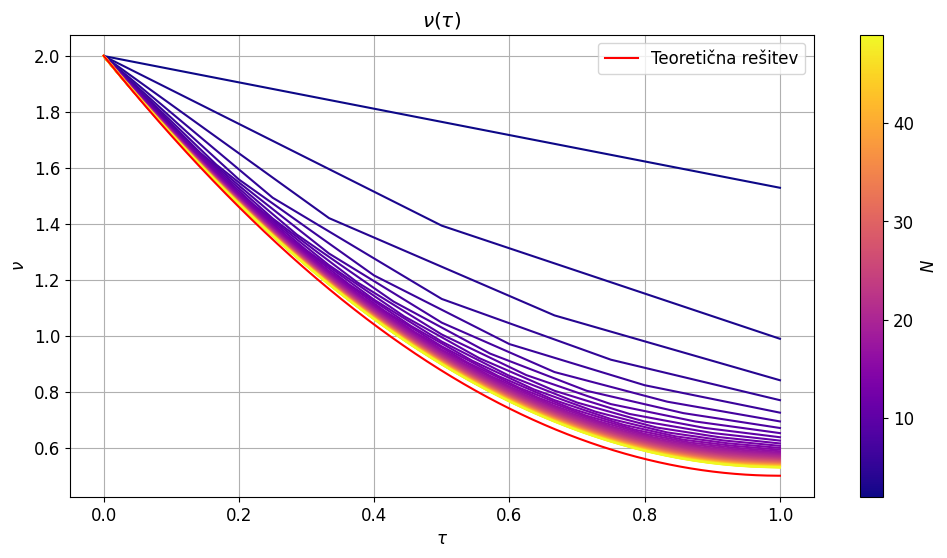
\includegraphics[width=12.5cm]{avto.png}
\caption{Optimalna vožnja avta $\nu(\tau)$ pridobljena z minimizacijo enačbe (14). Na grafu je z rdečo črto prikazana rešitev iz naloge 1.}
\end{figure}

Funkcional lahko silimo v določene rešitve še z veliko možnostmi. Poglejmo si le še usiljen pogoj za pozitivne hitrosti. Funkcionaloma $F_1$ in $F_2$ lahko prištejemo še

\begin{equation}
F_2 = \sum_{i=0}^{N} (1+e^{-\kappa_2 \nu_i)},
\end{equation}
ki bo rešitev minimizacije silil v pozitivne hitrosti. Tako v naslednjem koraku miniiziramo

\begin{equation}
F = F_1 + F_2 + F_3.
\end{equation}

Podoben učinek bi lahko dobili s določitvijo parametra \texttt{bounds} v funkciji \texttt{scipy.optimize.minimize}. Na sliki 11 je prikazan primer vožnje pri katerem se s pomočjo $F_2$ izognemo negativnim hitrostim. Za parameter $\kappa_2$ sem si izbral vrednost 100 in začetno hitrost $\nu_0 = 4$.

\begin{figure}[h!]
\centering
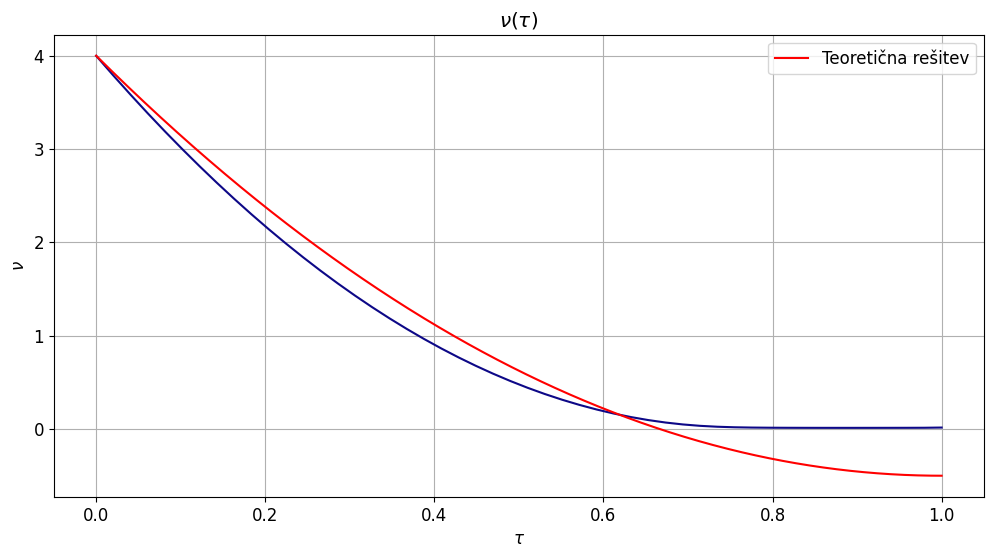
\includegraphics[width=12.5cm]{avto2.png}
\caption{Optimalna vožnja avta $\nu(\tau)$ pridobljena z minimizacijo enačbe (16). Na grafu je z rdečo črto prikazana rešitev iz naloge 1.}
\end{figure}

\section{Zaključek}

V nalogi smo reševali Thomsonov problem razmestitve nabojev po različnih telesih in likih ter problem optimalne vožnje z numerično minimizacijo.

Pri Thomsonovem problemu s sfero smo testirali lastnisti različnih numeričnih metod in predstavili prednosti vsake. Prav tako smo testirali metode s podanim gradientom funkcije in ugotovili, da se pri vsaki metodi to izplača. Grafično smo prikazali razporeditve nabojev na sferi, krogu, sferi v kondenzatorju, torusu in elipsoidu. Izmed izbranih likov in teles so rezultati povedali, da je naboje najbolj ugodno nalagati na izbrani torus in sfero.

V drugem delu naloge smo se vrnili k že znanemu problemu optimalne vožnje do semaforja in ga reševali z numerično minimizacijo. To smo lahko dosegli z diskretizacijo časa. Pogledali smo si različne manipulacije z funkcionalom in ga silili upoštevati različne pogoje oz. vezi. Rezultati so pokazali, da bolj kot diskretiziramo čas bolj natančen rezultat dobimo, kar me je presenetilo. Verjetno pri majhnih $N$-jih ne upoštevamo vezi o prevoženi poti najbolje, zaradi nizkega parametra $\kappa_1$. Nadaljno smo uspešno manipulirali funkcional v rešitev minimizacije brez negativnih hitrosti.

\end{document}